\begin{figure}[t]
\begin{center}
	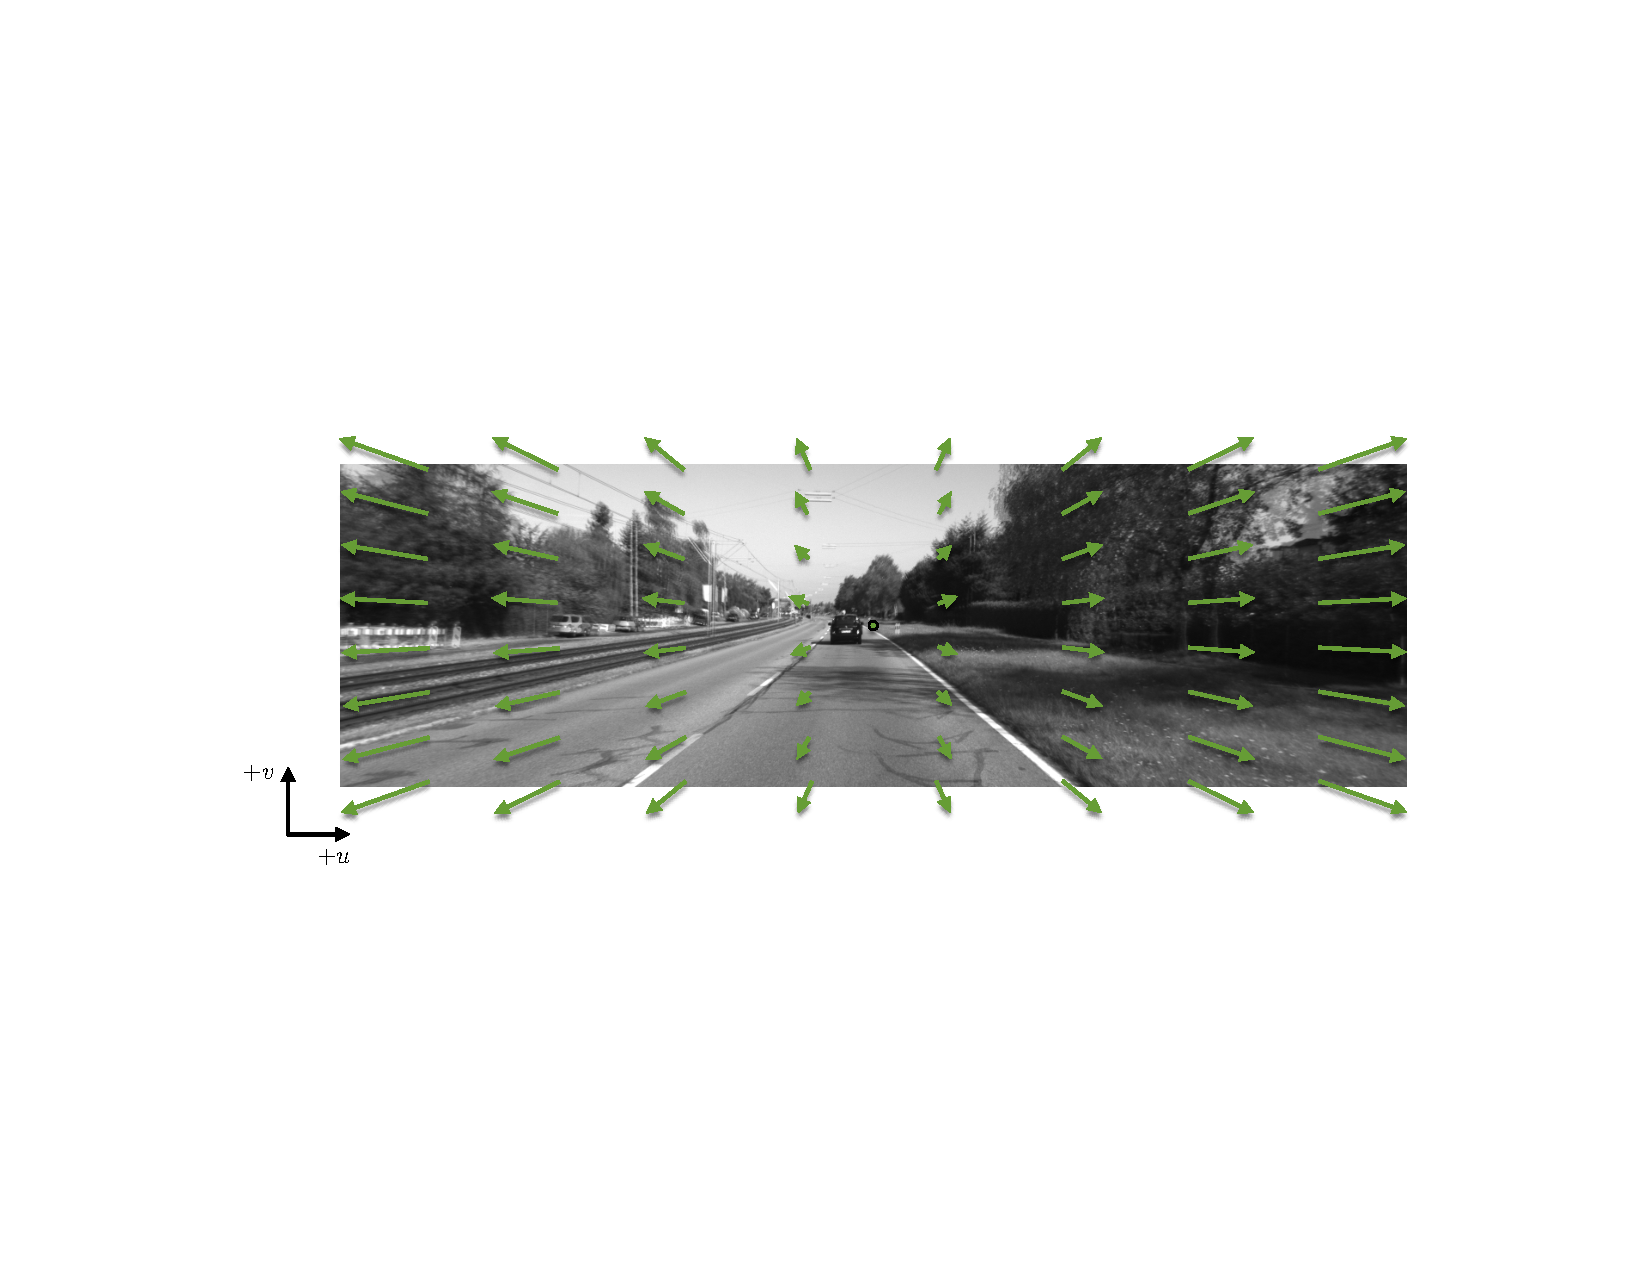
\epsfig{file=optical_flow.pdf, width = \textwidth}\\
	\caption[Optical flow visualization]{Optical flow visualization. Optical flow is a 2D displacement vector field used to represent the apparent motion of image pixels between two consecutive frames, caused by the movement of objects or the camera. Pictured are two, super-imposed, consecutive frames taken from the KITTI dataset \cite{geiger2013vision}. The corresponding optical flow is visualized as an array of green arrows. Note that this is just a sample of the motions that optical flow can characterize.}
	\vspace{-0.65cm}
	\label{fig:optical_flow}
\end{center}
\end{figure}